\documentclass[aspectratio=169,11pt]{beamer}

\usetheme[progressbar=frametitle]{metropolis}
\setbeamertemplate{frame numbering}[fraction]

\usepackage{amsmath,amssymb,mathtools}
\usepackage{bm}
\usepackage{dsfont}
\usepackage{mathrsfs}
\usepackage{xspace}
\usepackage{graphicx}
\usepackage{booktabs}

\DeclareMathOperator*{\argmin}{\arg\!\min}
\DeclareMathOperator*{\argmax}{\arg\!\max}
\DeclareMathOperator*{\E}{\mathbb{E}}
\DeclareMathOperator*{\Var}{Var}
\DeclareMathOperator*{\median}{median}
\DeclareMathOperator*{\mean}{mean}
\DeclareMathOperator{\supp}{supp}
\DeclareMathOperator{\esssup}{ess\,sup}
\DeclareMathOperator{\fastmobius}{FastMobius}
\DeclareMathOperator{\poly}{poly}
\DeclareMathOperator{\dec}{Dec}
\DeclareMathOperator{\sinc}{sinc}
\DeclareMathOperator{\linspan}{span}
\DeclareMathOperator{\proj}{Proj}
\DeclareMathOperator{\sv}{SV}
\DeclareMathOperator{\err}{err}
\DeclareMathOperator{\obj}{obj}
\DeclareMathOperator{\bern}{Bern}
\DeclareMathOperator{\binomdist}{Binom}
\DeclareMathOperator\erf{erf}

\newcommand{\type}[1]{\mathrm{Type} \left( #1 \right)}
\newcommand{\detect}[1]{\mathrm{Detect} \left( #1 \right)}

\newcommand{\abs}[1]{\left\lvert #1 \right\rvert}
\newcommand{\red}[1]{{\color{red}#1}}
\newcommand{\blue}[1]{{\color{blue}#1}}
\definecolor{lightpink}{rgb}{1,0.9,0.9}
\definecolor{figblue}{RGB}{0,100,200}
\definecolor{figred}{RGB}{200,50,50}
\definecolor{figgreen}{RGB}{0,140,60}
\definecolor{figpurple}{RGB}{150,50,150}
\newcommand{\defeq}{\vcentcolon=}
\newcommand{\eqdef}{=\vcentcolon}

\newcommand{\dt}{\text{ d}}
\newcommand{\calD}{\mathcal{D}}
\newcommand{\cA}{\mathcal A}
\newcommand{\cB}{\mathcal B}
\newcommand{\cC}{\mathcal C}
\newcommand{\cD}{\mathcal D}
\newcommand{\cE}{\mathcal E}
\newcommand{\cF}{\mathcal F}
\newcommand{\cG}{\mathcal G}
\newcommand{\cH}{\mathcal H}
\newcommand{\cI}{\mathcal I}
\newcommand{\cJ}{\mathcal J}
\newcommand{\cK}{\mathcal K}
\newcommand{\cL}{\mathcal L}
\newcommand{\cM}{\mathcal M}
\newcommand{\cN}{\mathcal N}
\newcommand{\cO}{\mathcal O}
\newcommand{\cP}{\mathcal P}
\newcommand{\cQ}{\mathcal Q}
\newcommand{\cR}{\mathcal R}
\newcommand{\cS}{\mathcal S}
\newcommand{\cT}{\mathcal T}
\newcommand{\cU}{\mathcal U}
\newcommand{\cV}{\mathcal V}
\newcommand{\cW}{\mathcal W}
\newcommand{\cX}{\mathcal X}
\newcommand{\cY}{\mathcal Y}
\newcommand{\cZ}{\mathcal Z}
\newcommand{\scrA}{\mathscr A}
\newcommand{\scrB}{\mathscr B}
\newcommand{\scrC}{\mathscr C}
\newcommand{\scrD}{\mathscr D}
\newcommand{\scrE}{\mathscr E}
\newcommand{\scrF}{\mathscr F}
\newcommand{\scrG}{\mathscr G}
\newcommand{\scrH}{\mathscr H}
\newcommand{\scrI}{\mathscr I}
\newcommand{\scrJ}{\mathscr J}
\newcommand{\scrK}{\mathscr K}
\newcommand{\scrL}{\mathscr L}
\newcommand{\scrM}{\mathscr M}
\newcommand{\scrN}{\mathscr N}
\newcommand{\scrO}{\mathscr O}
\newcommand{\scrP}{\mathscr P}
\newcommand{\scrQ}{\mathscr Q}
\newcommand{\scrR}{\mathscr R}
\newcommand{\scrS}{\mathscr S}
\newcommand{\scrT}{\mathscr T}
\newcommand{\scrU}{\mathscr U}
\newcommand{\scrV}{\mathscr V}
\newcommand{\scrW}{\mathscr W}
\newcommand{\scrX}{\mathscr X}
\newcommand{\scrY}{\mathscr Y}
\newcommand{\scrZ}{\mathscr Z}
\newcommand{\bbB}{\mathbb B}
\newcommand{\bbS}{\mathbb S}
\newcommand{\bbR}{\mathbb R}
\newcommand{\bbZ}{\mathbb Z}
\newcommand{\bbI}{\mathbb I}
\newcommand{\bbQ}{\mathbb Q}
\newcommand{\bbP}{\mathbb P}
\newcommand{\bbE}{\mathbb E}
\newcommand{\bbN}{\mathbb N}
\newcommand{\sfE}{\mathsf E}
\newcommand{\sfF}{\mathsf F}
\newcommand{\sfV}{\mathsf V}
\newcommand{\one}{\mathds 1}
\newcommand{\AND}{$\mathsf{AND}$\xspace}
\newcommand{\OR}{$\mathsf{OR}$\xspace}

\newcommand{\Tr}{ \text{Tr} }
\newcommand{\trans}{\textrm{T}}

\newcommand{\by}{\mathbf y}
\newcommand{\bxi}{\boldsymbol \xi}
\newcommand{\bx}{\mathbf x}
\newcommand{\bd}{\mathbf d}
\newcommand{\barbd}{\mathbf{ \overline{ d}}}
\newcommand{\barbh}{\mathbf{ \overline{ h}}}
\newcommand{\barbell}{\overline{ \mathbf{ \ell}}}
\newcommand{\bc}{\mathbf c}
\newcommand{\be}{\mathbf e}
\newcommand{\bg}{\mathbf g}
\newcommand{\bw}{\mathbf w}
\newcommand{\bW}{\mathbf W}
\newcommand{\bv}{\mathbf v}
\newcommand{\bj}{\mathbf j}
\newcommand{\bu}{\mathbf u}
\newcommand{\ba}{\mathbf a}
\newcommand{\bb}{\mathbf b}
\newcommand{\bk}{\mathbf k}
\newcommand{\boldm}{\mathbf m}
\newcommand{\br}{\mathbf r}
\newcommand{\bA}{\mathbf A}
\newcommand{\bM}{\mathbf M}
\newcommand{\bX}{\mathbf X}
\newcommand{\bY}{\mathbf Y}
\newcommand{\bD}{\mathbf D}
\newcommand{\bI}{\mathbf I}
\newcommand{\bH}{\mathbf H}
\newcommand{\bh}{\mathbf h}
\newcommand{\bs}{\mathbf s}
\newcommand{\bz}{\mathbf z}
\newcommand{\bS}{\mathbf S}
\newcommand{\bZ}{\mathbf Z}
\newcommand{\bU}{\mathbf U}
\newcommand{\bL}{\mathbf L}
\newcommand{\PASMT}{PASMT\xspace}
\newcommand{\FASMT}{FASMT\xspace}
\newcommand{\GBSA}{\text{GBSA}\xspace}
\newcommand{\bbeta}{\bm \beta}
\newcommand{\balpha}{\bm \alpha}
\newcommand{\bell}{\boldsymbol{\ell}}
\newcommand{\bZero}{\boldsymbol 0}
\newcommand{\bOne}{\boldsymbol 1}
\newcommand{\beps}{\boldsymbol{\epsilon}}
\newcommand{\indep}{\perp \!\!\! \perp}



\title{Adaptive Sparse M\"obius Transforms\\for Learning Polynomials}
\author{Yigit Efe Erginbas \and Justin Kang \and Elizabeth Polito \and Kannan Ramchandran}
\institute{University of California, Berkeley}
\date{}

\begin{document}

\maketitle

%=====================================================================
\section{Introduction}
%=====================================================================

\begin{frame}{Motivation: reconstructing hidden combinatorial structure}
  \begin{center}
    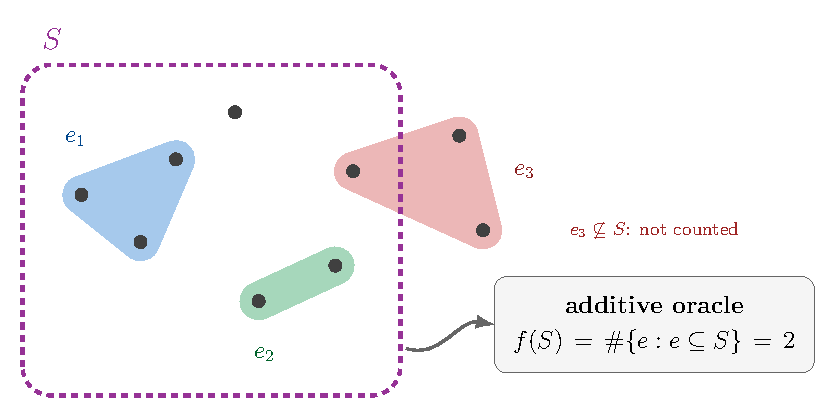
\includegraphics[width=0.64\textwidth]{figures/fig_hypergraph.pdf}
  \end{center}
  \begin{itemize}
    \item Hidden hypergraph: circuits, metabolic networks, communities, \dots
    \item We may ask \alert{additive queries}: how many hyperedges inside $S$?
    \item Goal: \alert{exact} reconstruction with as few queries as possible.
  \end{itemize}
\end{frame}

\begin{frame}{From hypergraphs to sparse polynomials}
  Encode the queried vertex subset as $\bx \in \{0,1\}^n$. The additive oracle is a \alert{polynomial}:
  \begin{equation*}
    f(\bx) \;=\; \sum_{\bk \leq \bx} F(\bk)
    \qquad \text{--- sum of weights $F(\bk)$ of hyperedges $\bk$ inside the queried set}
  \end{equation*}
  \vspace{-1ex}
  \begin{itemize}
    \item $s$ hyperedges of size $\le d$ \;$\Leftrightarrow$\; \textbf{$s$-sparse} polynomial of \textbf{degree $d$}.
  \end{itemize}
  \vspace{1ex}
  \begin{alertblock}{Goal: sparse M\"obius transform}
    Exactly recover all pairs $(\bk, F(\bk))$ from few evaluation queries $f(\bx)$.
  \end{alertblock}
\end{frame}

\begin{frame}{Why not Fourier analysis?}
  \begin{center}
    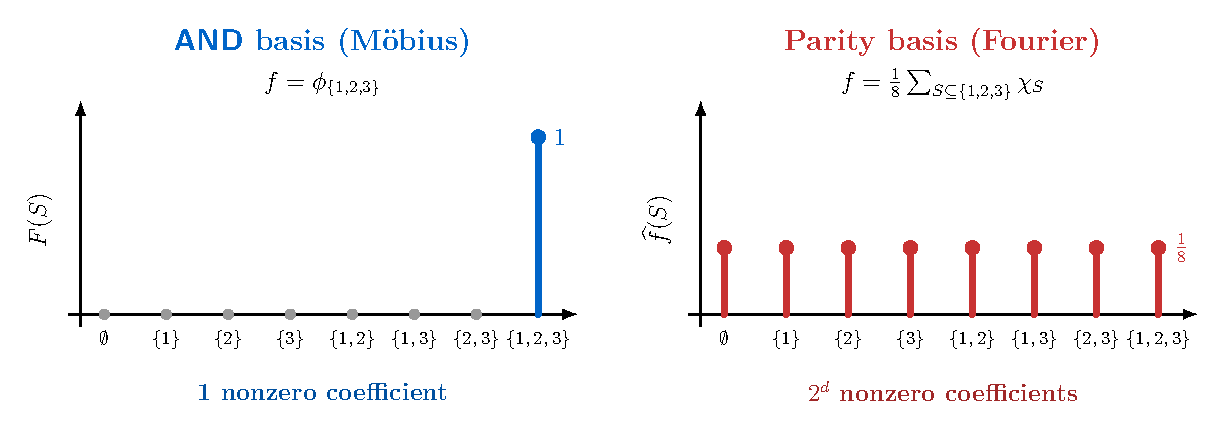
\includegraphics[width=0.8\textwidth]{figures/fig_mismatch.pdf}
  \end{center}
  \centering
  Conjunctions are \alert{local}; parities are \alert{global}.\\
  Fourier-based methods (cut queries) must pay $2^d$ for a single size-$d$ hyperedge.
\end{frame}

\begin{frame}{Prior approaches: every query model hits a barrier}
  \begin{center}
    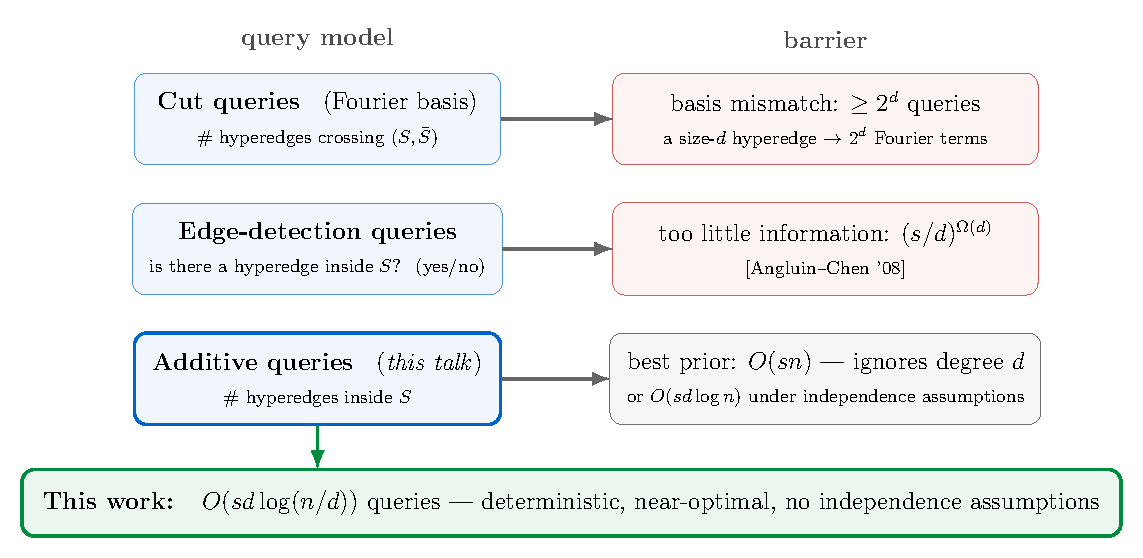
\includegraphics[width=0.8\textwidth]{figures/fig_oracles.pdf}
  \end{center}

\end{frame}

\begin{frame}{Our results}
  \begin{block}{\FASMT{} \; (fully adaptive)}
    $O(sd \log (n/d))$ queries, polynomial time \hfill \alert{near-optimal}
  \end{block}
  \begin{block}{\PASMT{} \; (partially adaptive)}
    $O(sd^2 \log n)$ queries in only $O(d^2 \log n)$ rounds \hfill \alert{rounds independent of $s$}
  \end{block}
  \begin{block}{Lower bound}
    $\Omega\bigl(sd\log(n/d)/\log s\bigr)$ queries required by \emph{any} algorithm
  \end{block}
  \vspace{1ex}
  \centering
  Deterministic, constructive, no independence assumptions.
\end{frame}

%=====================================================================
\section{Queries are Group Tests}
%=====================================================================

\begin{frame}{Evaluations are group tests over the Boolean semiring}
  \begin{align*}
    f(\bx) &= \sum_{\bk \leq \bx} F(\bk)
      && \text{evaluation = subset sum} \\[1ex]
    \bk \leq \bx \;\; &\Longleftrightarrow \;\; \bh^\top \bk = 0, \quad \bh \defeq \neg\bx
      && \text{\alert{group test} on the support of $F$} \\[1ex]
    f(\bOne) - f(\neg\bh) &= \sum_{\bh^\top \bk = 1} F(\bk), \qquad
    f(\neg\bh) = \sum_{\bh^\top \bk = 0} F(\bk)
      && \text{one query splits the space}
  \end{align*}
  \vspace{0.5ex}
  \begin{alertblock}{Key insight}
    Group testing designs act as \emph{projections of the coefficient space}:\\
    we can navigate the subset lattice by iteratively splitting with test vectors $\bh$.
  \end{alertblock}
\end{frame}

\begin{frame}{Divide and conquer on the coefficient space}
  Split coefficients into \alert{bins} by test outcomes: starting from $\cB(\beps) = \{0,1\}^n$,
  \begin{equation*}
    \cB(\bell \| 0) = \{\bk \in \cB(\bell) : \bh^\top \bk = 0\}, \qquad
    \cB(\bell \| 1) = \{\bk \in \cB(\bell) : \bh^\top \bk = 1\}
  \end{equation*}
  with \alert{bin sums} $V(\bell) = \sum_{\bk \in \cB(\bell)} F(\bk) = V(\bell\|0) + V(\bell\|1)$.
  \vspace{1ex}
  \begin{itemize}
    \item \textbf{Prune}: $V(\bell) = 0 \;\Rightarrow\;$ discard $\cB(\bell)$.\footnote{Safe under a
      mild non-degeneracy assumption (e.g., satisfied almost surely by random weights).}
    \item \textbf{Peel}: single coefficient left $\Rightarrow$ value $=$ bin sum, location $=$ outcomes $\bell$.
    \item Tree has width $\le s$ (sparsity) --- pruning keeps the search small.
  \end{itemize}
\end{frame}

\begin{frame}{The catch: queries mix bins}
  No query isolates a single bin. The best we can do (query vector $\bx_{\bell}$):
  \begin{equation*}
    f(\bx_{\bell}) \;=\; \sum_{\bH^\top \bk \,\leq\, \bell} F(\bk)
    \qquad \text{--- the target bin \alert{plus} all bins below it}
  \end{equation*}
  \vspace{1ex}
  \begin{columns}[T]
    \begin{column}{0.48\textwidth}
      \begin{block}{\PASMT: shared tests}
        Fixed matrix $\bH$ for all bins\\
        $\Rightarrow$ structured linear system,\\
        solve all bin sums per round
      \end{block}
    \end{column}
    \begin{column}{0.48\textwidth}
      \begin{block}{\FASMT: adaptive tests}
        Per-bin test vectors\\
        $\Rightarrow$ process bins in order,\\
        subtract already-found coefficients
      \end{block}
    \end{column}
  \end{columns}
\end{frame}

%=====================================================================
\section{Two Algorithms}
%=====================================================================

\begin{frame}{\PASMT: breadth-first splitting with a fixed design}
  \begin{center}
    \only<1>{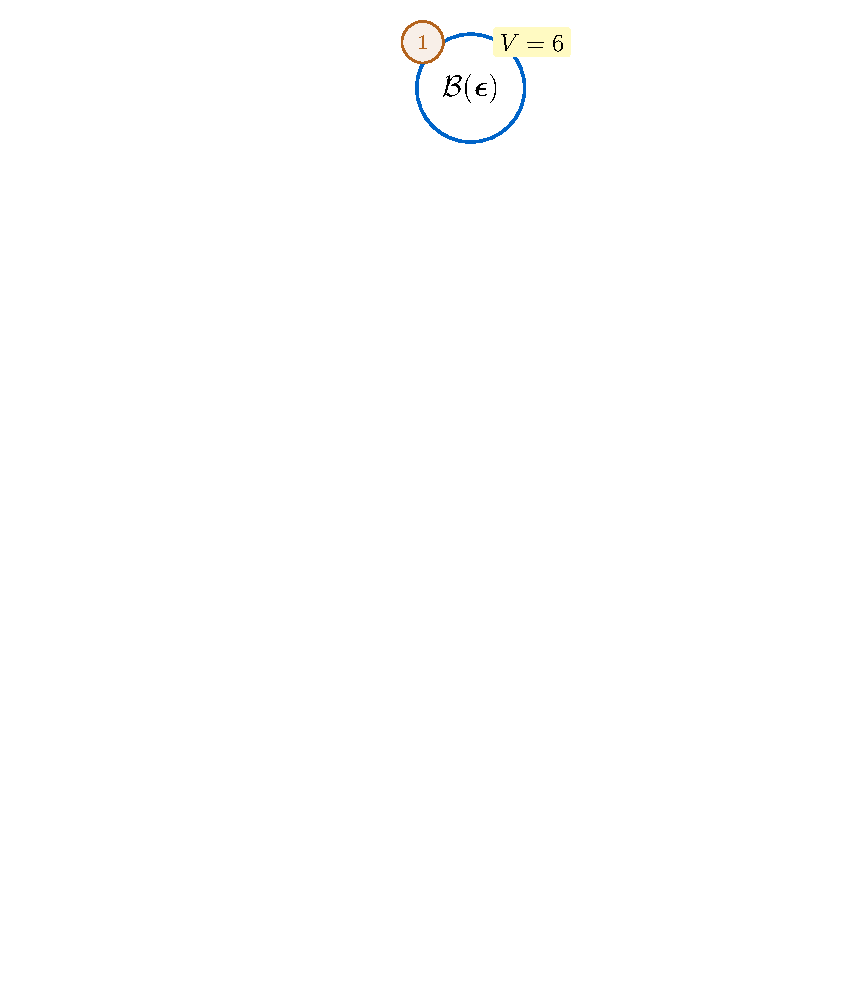
\includegraphics[height=0.7\textheight,page=1]{figures/fig_pasmt_tree.pdf}}%
    \only<2>{\includegraphics[height=0.7\textheight,page=2]{figures/fig_pasmt_tree.pdf}}%
    \only<3>{\includegraphics[height=0.7\textheight,page=3]{figures/fig_pasmt_tree.pdf}}%
    \only<4>{\includegraphics[height=0.7\textheight,page=4]{figures/fig_pasmt_tree.pdf}}%
    \only<5>{\includegraphics[height=0.7\textheight,page=5]{figures/fig_pasmt_tree.pdf}}%
  \end{center}
  \centering\small
  All bins at depth $t$ split with the \alert{same} column $\bh_t$ of a $d$-disjunct matrix $\bH$.
\end{frame}

\begin{frame}{\PASMT: why it works}
  \begin{itemize}
    \item $\bH$: \alert{$d$-disjunct} group testing matrix with $b = O(d^2 \log n)$ columns.
    \item Each round: queries form a \alert{lower-triangular} linear system in the bin sums\\
          $\Rightarrow$ back-substitution recovers every active bin, one query per bin.
    \item After $b$ rounds each surviving bin holds one coefficient;\\
          location decoded from its label: $\bell = \bH^\top \bk \;\Rightarrow\; \bk = \textsc{Decode}(\bH, \bell)$.
  \end{itemize}
  \vspace{1ex}
  \begin{alertblock}{Theorem (\PASMT)}
    Exact recovery with $O(sd^2 \log n)$ queries in $O(d^2\log n)$ \emph{rounds} ---
    independent of $s$.
  \end{alertblock}
\end{frame}

\begin{frame}{\FASMT: depth-first search with adaptive tests}
  \begin{center}
    \only<1>{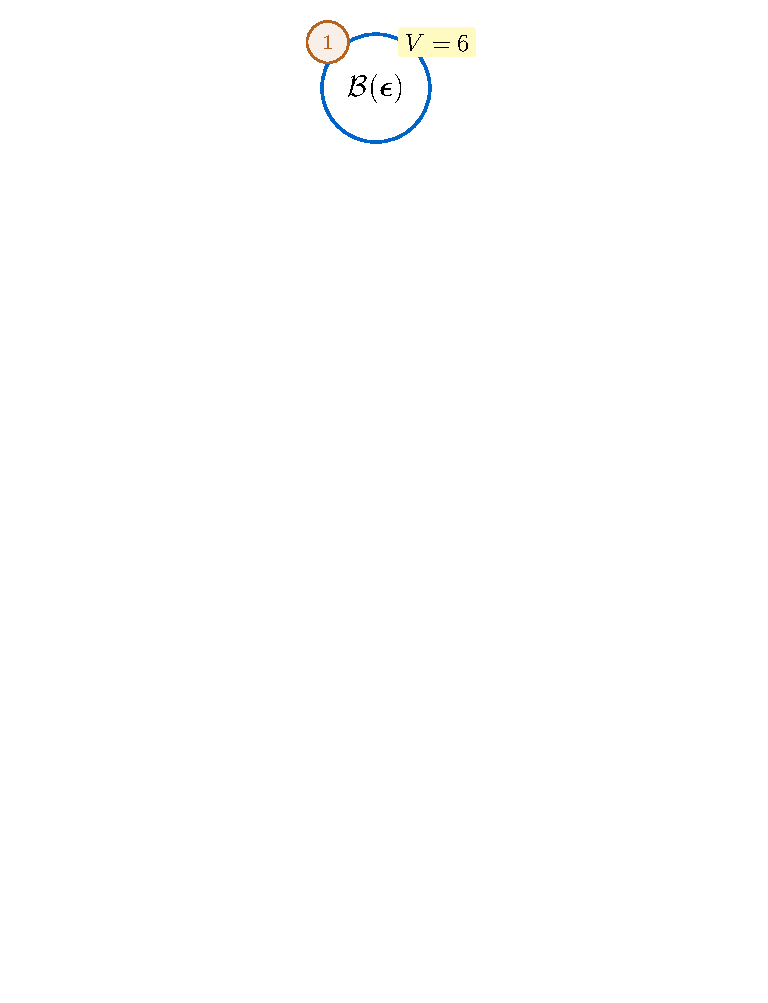
\includegraphics[height=0.7\textheight,page=1]{figures/fig_fasmt_tree.pdf}}%
    \only<2>{\includegraphics[height=0.7\textheight,page=2]{figures/fig_fasmt_tree.pdf}}%
    \only<3>{\includegraphics[height=0.7\textheight,page=3]{figures/fig_fasmt_tree.pdf}}%
    \only<4>{\includegraphics[height=0.7\textheight,page=4]{figures/fig_fasmt_tree.pdf}}%
    \only<5>{\includegraphics[height=0.7\textheight,page=5]{figures/fig_fasmt_tree.pdf}}%
    \only<6>{\includegraphics[height=0.7\textheight,page=6]{figures/fig_fasmt_tree.pdf}}%
    \only<7>{\includegraphics[height=0.7\textheight,page=7]{figures/fig_fasmt_tree.pdf}}%
  \end{center}
  \centering\small
  Test vectors chosen \alert{adaptively} per bin by generalized binary splitting (\GBSA{}).
\end{frame}

\begin{frame}{\FASMT: why it works}
  \begin{itemize}
    \item \GBSA{} [Hwang '72] pins down a $\le d$-sparse $\bk$ in $O(d\log(n/d))$ tests\\
          $\Rightarrow$ only $O(d \log (n/d))$ splits per coefficient (vs.\ $O(d^2 \log n)$ fixed tests).
    \item Adaptive tests break the linear-system structure.\\
          Fix: process bins \alert{depth-first} and query the \alert{residual}
          \begin{equation*}
            f_T(\bx) = f(\bx) - \sum_{\bk \leq \bx} T(\bk), \qquad T = \text{coefficients found so far,}
          \end{equation*}
          so each split still costs a \alert{single} query.
  \end{itemize}
  \begin{alertblock}{Theorem (\FASMT)}
    Exact recovery with $O(sd \log(n/d))$ queries, in polynomial time.
  \end{alertblock}
\end{frame}

\begin{frame}{Two ends of an adaptivity trade-off}
  \begin{center}
  \renewcommand{\arraystretch}{1.35}
  \begin{tabular}{lcc}
    \toprule
     & \PASMT & \FASMT \\
    \midrule
    traversal & breadth-first & depth-first \\
    test vectors & fixed $d$-disjunct $\bH$ & adaptive (\GBSA) \\
    queries & $O(sd^2\log n)$ & $\alert{O(sd\log (n/d))}$ \\
    adaptive rounds & $\alert{O(d^2\log n)}$ & $O(sd\log (n/d))$ \\
    \bottomrule
  \end{tabular}
  \end{center}
  \vspace{1.5ex}
  \centering
  Choose by bottleneck: total measurements (\FASMT) vs.\ parallelism (\PASMT).
\end{frame}

%=====================================================================
\section{Lower Bound}
%=====================================================================

\begin{frame}{\FASMT{} is near-optimal}
  Counting argument:
  \begin{itemize}
    \item Many candidates: describing $f$ takes $\Omega(sd \log(n/d))$ bits.
    \item Little information per query: each answer reveals only $O(\log s)$ bits.
  \end{itemize}
  \vspace{1ex}
  \begin{alertblock}{Theorem (lower bound)}
    Any deterministic algorithm needs
    $\;\Omega\!\left(\dfrac{sd\log(n/d)}{\log s}\right)\;$ evaluation queries.
  \end{alertblock}
  \vspace{1ex}
  \centering
  \FASMT{}'s $O(sd\log(n/d))$ matches up to $O(\log s)$ --- in \emph{every} scaling regime of $s, d$.
\end{frame}

%=====================================================================
\section*{Conclusion}
%=====================================================================

\begin{frame}{Takeaways \& open questions}
  \begin{block}{Takeaways}
    \begin{itemize}
      \item M\"obius (\AND) basis keeps conjunctive structure sparse --- and group testing\\
            turns evaluation queries into a constructive search over the coefficient lattice.
      \item \FASMT: near-optimal $O(sd\log(n/d))$; \PASMT: few rounds, independent of $s$.
    \end{itemize}
  \end{block}
  \begin{block}{Open questions}
    \begin{itemize}
      \item Noisy oracles --- import robust group testing?
      \item Fewer adaptive rounds at $O(sd\log n)$ queries?
      \item Is the non-cancellation assumption necessary?
    \end{itemize}
  \end{block}
  \vspace{1ex}
  \centering \alert{Thank you!}
\end{frame}

\end{document}
